%!TEX root = ../crimson_throne_book_main.tex
% 2015-02-15
The companions take the rest of the day to recover from their ordeal at the hands of the Graul family. They consider burning down the hunting lodge, but despite the horror that the ogrekin brought to the place, it is a decent and sturdily built edifice. In the end the heroes decide to spare the building and burn the corpses outside on a large funeral pyre instead. Dernal, the satyr they saved, and Quint's horse seem to have withstood the worse of the trauma. The goat-legged man leaves for the forest to rejoin his kin, nodding his head in gratitude one last time and Quint's riding animal seeks comfort among his three brothers.\\

\section{4 Erastus 4708}

You might recognize Lost End, the abandoned Porphyria manor, as my version of Foxglove Manor, a.k.a. Misgivings, from The journey to Lost End takes just under three hours. The smell of the sea air and the cry of seagulls are the first signs that the companions are nearing their destination. Perched high above the ocean, on the edge of the cliffs, rests a stately manor house. Strong winds tear at the structure that looks poised for a suicide leap. That the manor clings to the top of the rocks is remarkable, as its far side hangs over a sheer drop down to the ocean below, a fall of over three hundred feet. The roof sags in several places and mold and mildew cake the walls. The house is crooked, its chimneys rise from various points among the rooftops, leaning like old men against the storm.\\

Four grinning gargoyles guard the front door and come to life when the companions approach. The demonic statues spread their stony wings and swoop down on the visitors. The heroes organize their defenses well and focus their attacks on one creature at a time, making short work of their enemies and minimizing the damage they take themselves. Since they have burned through every potion and wand that provides healing, they have to be careful with their resources, as only Sjo's and Quint's spells can cure wounds now.\\

The front door is barred from the inside, but the {\itshape Key-Lock Killer's bell} easily takes care of that obstacle. The entrance hall is \hyperref[fig:Pathfinder-Foxglove-manor-to-Lost-End-ground-floor-513919727]{ large and runs through to another room at the end of the house } , from where colored light streams in through beautiful stained-glass windows. A twelve-foot long monster towers over the visitors as they enter: its leathery wings spread out menacingly. The creature has the body of a giant lion, though its feline head is flanked by two more heads - a dragon's and a horned goat's - marking it as a chimera. The heroes draw their weapons before realizing that this fabled beast is not moving. It is a stuffed animal, a \hyperref[fig:Pathfinder-Foxglove-manor-to-Lost-End-chimera-513923128]{ magnificent trophy } from a long forgotten battle. The entrance hall sports other trophies along its walls, the heads of bears, boars and giant deer mounted on wooden display plaques. A lion's pelt covers the floor leading to the dining room in the back. A curving flight of stairs to the right winds up to the upper floor, and several doors provide entry to other rooms, their frames carved with scenes from the forest, the animals that inhabit the wilds and the hunters that chase them down. The house is definitely dirty, but the mold staining the floor, walls and ceiling does not carry the damp smell of decay that fifty years of degeneration should, suggesting that the place was aired not too long ago. Still, there are no signs of life anywhere now. The dining room in the back holds a large mahogany table. The cups and plates on it also show signs of recent use, no more than a couple of weeks ago. The stained glass in the windows is still intact and looks like excellent craftsmanship, but the colored glass blocks most of what would have been a breathtaking view of the Bay of Korvosa. \\

\begin{figure}[h]
	\centering
	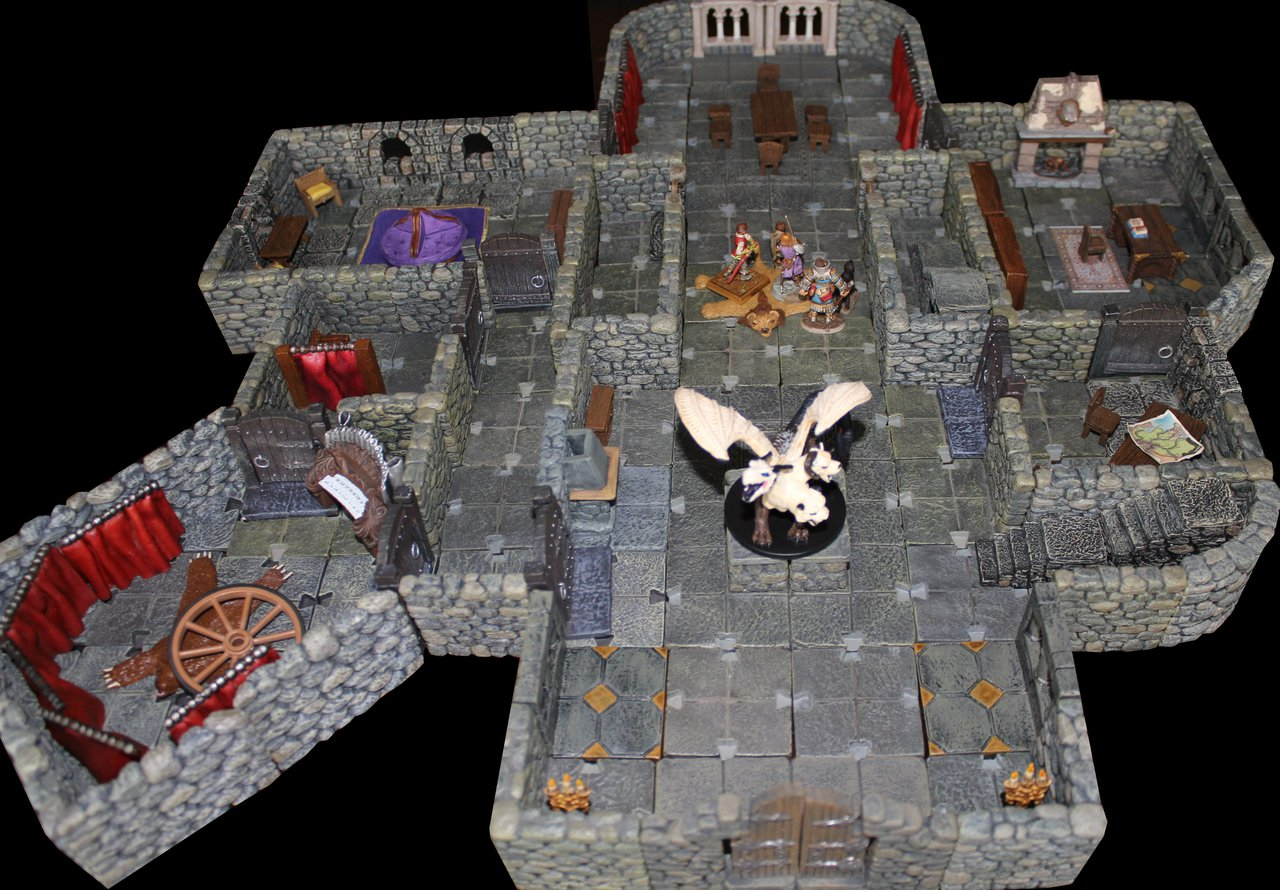
\includegraphics[width=0.39\textwidth]{images/Pathfinder-Foxglove-manor-to-Lost-End-ground-floor-513919727.jpg}
	\caption{Pathfinder Foxglove manor to Lost End ground floor}
	\label{fig:Pathfinder-Foxglove-manor-to-Lost-End-ground-floor-513919727}
\end{figure}

\begin{figure}[h]
	\centering
	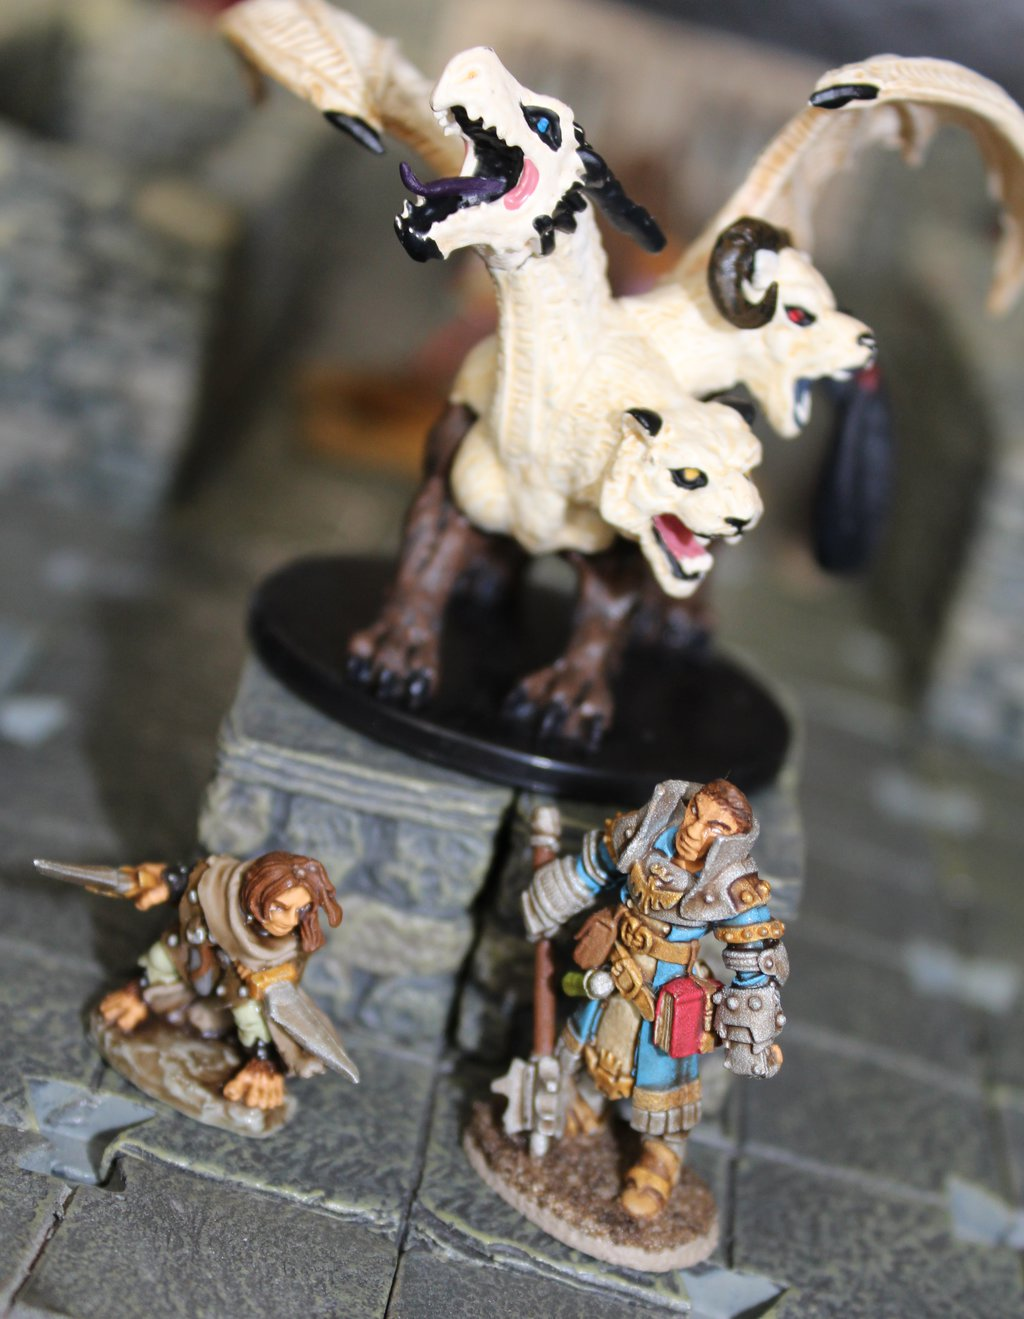
\includegraphics[width=0.39\textwidth]{images/Pathfinder-Foxglove-manor-to-Lost-End-chimera-513923128.jpg}
	\caption{Pathfinder Foxglove manor to Lost End chimera}
	\label{fig:Pathfinder-Foxglove-manor-to-Lost-End-chimera-513923128}
\end{figure}

The companions make their way through the rest of the ground floor, including a dusty lounge and a\hyperref[fig:Pathfinder-Foxglove-manor-to-Lost-End-music-room-513922417]{ ruined music room } . The once-magnificent chandelier lies smashed on the floor, although the organ in the corner survived the crash. Still, half a century of disuse has not been kind on the instrument, which only produces false notes. The drawing room and library are cleaner and have obviously seen more use recently. The heroes discover notes on how to construct a flesh golem, including the creature's strengths and 'weaknesses'. The instructions also list the magic required to bring such a golem to life, with hard to find spells like  {\itshape geas} and  {\itshape limited wish} . The first would apparently be provided by someone called Andaisin, while the latter would come from a scroll. Quint suspects that these scribblings belonged to Rolth, the necromancer who took Balian's sister five years ago. \\

\begin{figure}[h]
	\centering
	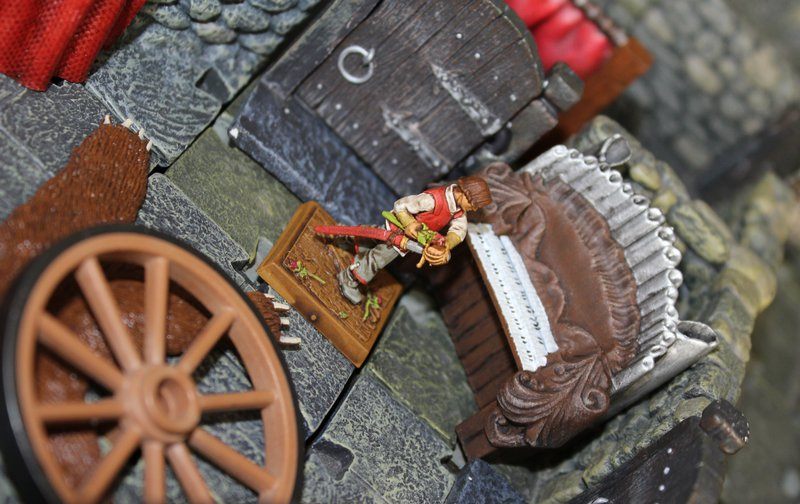
\includegraphics[width=0.39\textwidth]{images/Pathfinder-Foxglove-manor-to-Lost-End-music-room-513922417.jpg}
	\caption{Pathfinder Foxglove manor to Lost End music room}
	\label{fig:Pathfinder-Foxglove-manor-to-Lost-End-music-room-513922417}
\end{figure}

Sjo rummages through more molded novels that are left on the bookshelves and some papers on the desk. He finds a document entitled the {\itshape plague plan} , that details the procedure on how to approach the Korvosa with  {\itshape the Delivery} . All passengers would leave the ship aboard rowing boats and make for the south of the city, while one person, named 'Rois', would stay on board and navigate the vessel into the mouth of the Jeggare River, where he would release the diseased rats, sink the boat and burn the evidence. The author of the note clearly had little respect for the suicide navigator, as he mocks the man for a fool. On\hyperref[fig:Pathfinder-Foxglove-manor-to-Lost-End-upper-floor-513924264]{ the upper floor of Lost End } the heroes discover a shrine to Urgathoa in the room above the dining room. \hyperref[fig:Pathfinder-Foxglove-manor-to-Lost-End-undead-513925444]{ Four skeletal warriors guard the unholy altar. } They throw themselves at the intruders, but like the gargoyles at the front door, they go down relatively easily, though not without delivering some vicious cuts with their rusted blades. Sjo heals his friends after the fight, but decides against patching up Spyder. The labrador sustained some gaping wounds and curing him would drain too many resources, so the companions leave the dog to guard the front door instead. The focal point in the improvised shrine is a statue of Urgathoa in front of the stained glass windows. Closer inspection reveals that this idol is actually a stone bust of a woman, named 'Lady Ulrika Porphyria', to which a skeletal lower body and arms were added. \\

\begin{figure}[h]
	\centering
	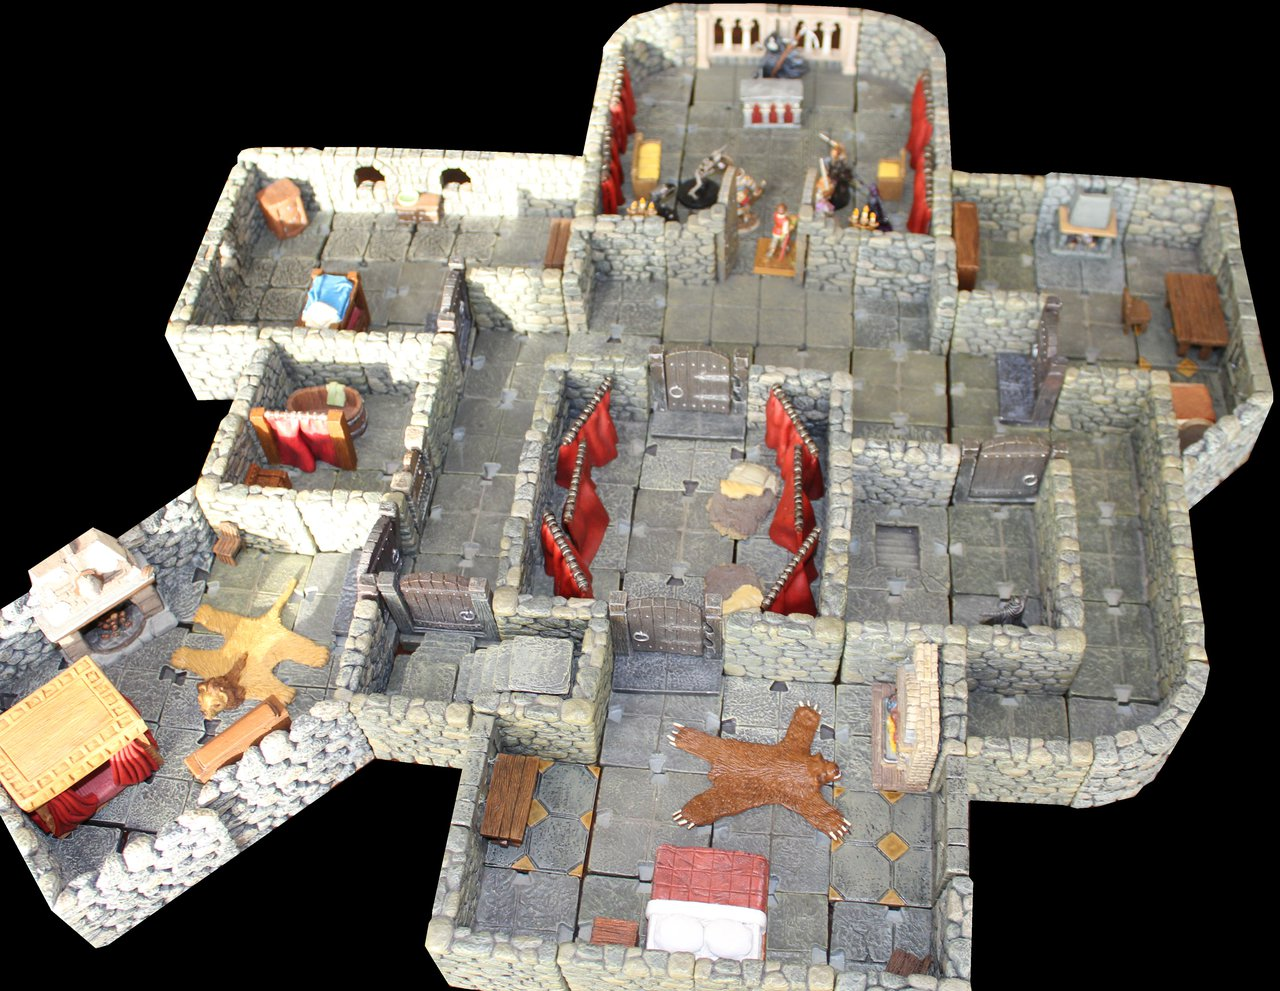
\includegraphics[width=0.39\textwidth]{images/Pathfinder-Foxglove-manor-to-Lost-End-upper-floor-513924264.jpg}
	\caption{Pathfinder Foxglove manor to Lost End upper floor}
	\label{fig:Pathfinder-Foxglove-manor-to-Lost-End-upper-floor-513924264}
\end{figure}

\begin{figure}[h]
	\centering
	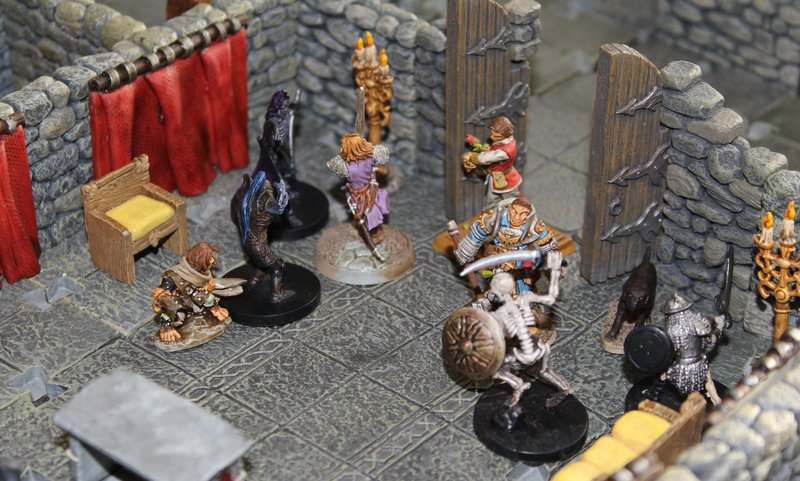
\includegraphics[width=0.39\textwidth]{images/Pathfinder-Foxglove-manor-to-Lost-End-undead-513925444.jpg}
	\caption{Pathfinder Foxglove manor to Lost End undead}
	\label{fig:Pathfinder-Foxglove-manor-to-Lost-End-undead-513925444}
\end{figure}

